\documentclass[]{politex}

% ========== Packages ==========
\usepackage[utf8]{inputenc}
\usepackage{amsmath,amsthm,amsfonts,amssymb}
\usepackage{graphicx,cite,enumerate}
\graphicspath{ {images/}{../images/} }
\usepackage{tabularx}
\usepackage{longtable}
\usepackage{subfiles}
\usepackage{subcaption}
\usepackage{multirow}
\usepackage{float}
\usepackage[table,xcdraw]{xcolor}
\usepackage{listings}
\usepackage{pdfpages}
\usepackage{booktabs}

% ========== Language options ==========
\usepackage[brazil]{babel}
%\usepackage[english]{babel}


% ========== ABNT (requer ABNTeX 2) ==========
%	http://www.ctan.org/tex-archive/macros/latex/contrib/abntex2
\usepackage[num]{abntex2cite}

% Forçar o abntex2 a usar [ ] nas referências ao invés de ( )
\citebrackets{[}{]}


% ========== Lorem ipsum ==========
\usepackage{blindtext}

% ========== Opções do documento ==========
% Título
\titulo{Rede de Dispositivos para Monitoramento de qualidade e conforto em escritórios}

% Autor
\autor{Isabella Bologna Salomão\\%
		Renato de Oliveira Freitas}


% Orientador / Coorientador
\orientador{Prof. Dr. Gustavo P. Rehder\\%
			Prof.ª Dra. Cíntia Borges Margi}
% \coorientador{PullUp \\%
%             Eng. Conrado Leite de Vitor }

% Tipo de documento
% \tcc{Eletricista com ênfase em Eletrônica e Sistemas}
\tcc{Eletricista com ênfase em Computação}
% \dissertacao{Engenharia Elétrica}
%\teseDOC{Engenharia Elétrica}
%\teseLD
%\memorialLD

% Departamento e área de concentração
\departamento{PSI - Eletrônica e Sistemas}
\departamento{PCS - Computação e Sistemas Digitais}
\areaConcentracao{Engenharia Elétrica}


% Local
\local{São Paulo}

% Ano
\data{2020}


\begin{document}
% ========== Capa e folhas de rosto ==========
\capa

\falsafolhaderosto

\folhaderosto
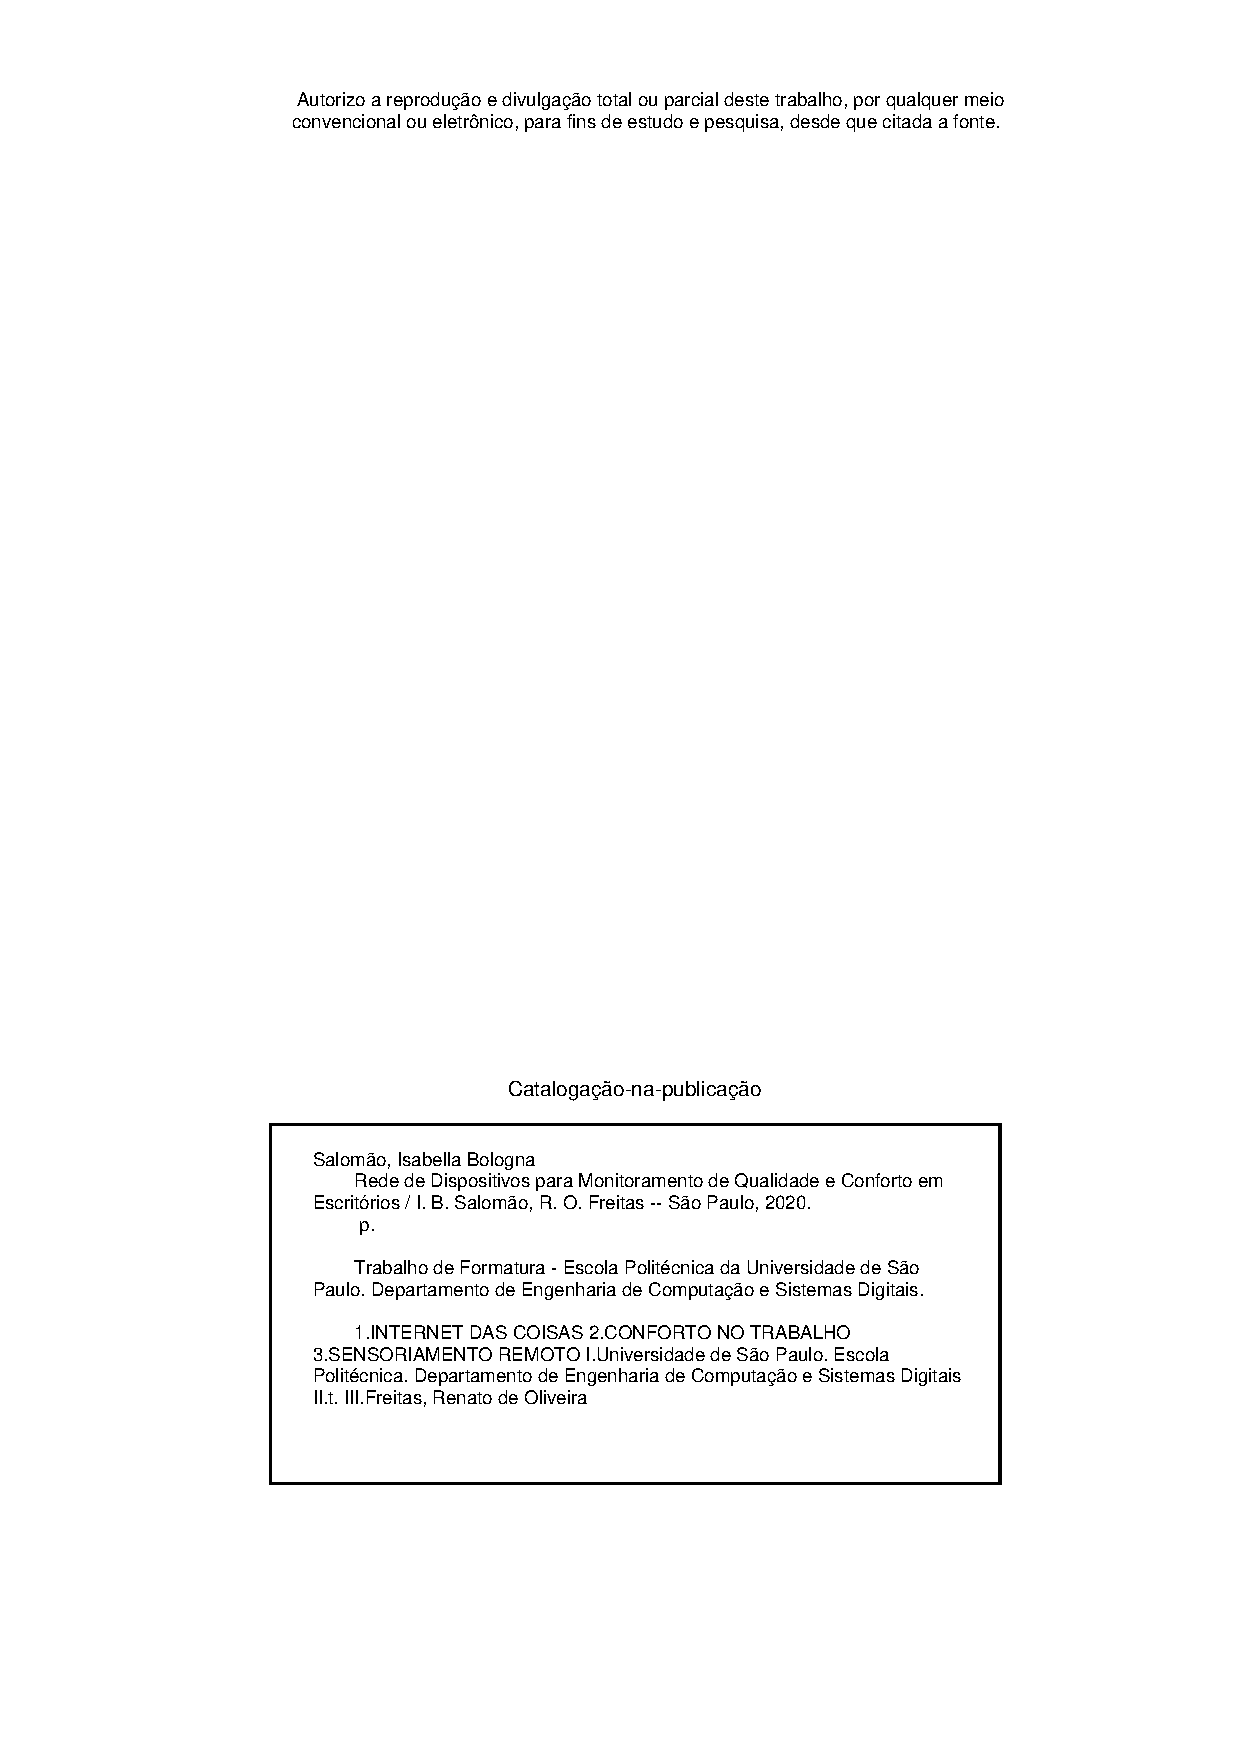
\includepdf{EPUSP-Catalogacao-na-Fonte.pdf}


% ========== Resumo ==========
\begin{resumo}
Soluções para o monitoramento de parâmetros que remetem à qualidade e conforto de ambientes internos vêm se tornando interessantes, dado o aumento no tempo que pessoas passam nesse tipo de ambiente, como escritórios. A partir da coleta desses dados, é possível adotar medidas para tornar o local estudado mais saudável e confortável para as pessoas ali presentes. O objetivo desse trabalho é desenvolver uma rede de dispositivos eletrônicos \textit{Open Source} capaz de monitorar escritórios fechados, realizando a medição através de sensores de dados referentes à qualidade do ar, temperatura, luminosidade e ruído, e coletando a opinião das pessoas sobre sua sensação de conforto no ambiente, para apresentar relatórios sobre o local em uma plataforma a fim de tomar ações para garantir o conforto de seus ocupantes. 
%
\\[3\baselineskip]
%
\textbf{Palavras-Chave} -- Internet of Things, Conforto Térmico, Conforto Acústico, Conforto Luminoso, Qualidade do Ar, Wireless Sensor Network, Green Buildings, Smart Office.
\end{resumo}

% ========== Listas (opcional) ==========
% \listadefiguras
% \listadetabelas


% ========== Sumário ==========
\sumario

% ========== Elementos textuais ==========

\chapter{Introdução}
\subfile{chapters/introducao}

\chapter{Estado da Arte e Trabalhos Relacionados} % Tema? ~Estado da Arte~
\subfile{chapters/arte}

\chapter{Especificação}
\subfile{chapters/specs}

\chapter{Desenvolvimento}
\subfile{chapters/dev}

\chapter{Verificação do Projeto}
\subfile{chapters/resultados}

\chapter{Considerações Finais}
\subfile{chapters/conclusao}

\appendix
\chapter{Imagens}
\subfile{chapters/anexo}


% ========== Referências ==========
% --- IEEE ---
%	http://www.ctan.org/tex-archive/macros/latex/contrib/IEEEtran
%\bibliographystyle{IEEEbib}

% --- ABNT (requer ABNTeX 2) ---
%	http://www.ctan.org/tex-archive/macros/latex/contrib/abntex2
\bibliographystyle{abntex2-num}

\bibliography{reference}

\end{document}